\chapter{Specific requirements}

\section{External interface requirements}
\subsection{User Interfaces}
\subsection{Hardware Interfaces}
The platform requires a device with a web browser to be accessed.
\subsection{Software Interfaces}
S\&C is a web application that requires a web browser to be accessed.
\subsection{Communication Interfaces}
All the communication between the platform and the users is done through the web application via HTTPS.

\section{Functional requirements}

\subsection{Use cases}

\subsubsection{StudentSignsUp}

\begin{table}[H]
    \centering
    \begin{tabular}{|l|m{10cm}|}
        \hline \multicolumn{2}{|c|}{\textbf{StudentSignsUp}} \\
        \hline \textbf{Actor} & Student, Students\&Companies, EmailService \\
        \hline \textbf{Entry condition} & The student is not already registered \\
        \hline \textbf{Event flow} &
            \begin{enumerate}
                \item The student opens the sign up page
                \item The platform shows the sign up page
                \item The student fills in the required informations and clicks the sign up button
                \item The platform checks that the information provided is valid
                \item The platform sends an email through the email service to verify the student account
                \item The student verifies the account
                \item The platform registers the new student account
                \item The platform shows the student profile page
            \end{enumerate} \\
        \hline \textbf{Exit condition} & The student is registered \\
        \hline \textbf{Exceptions} & The student is already registered \\
        \hline
    \end{tabular}
\end{table}

\begin{figure}[H]
    \centering
    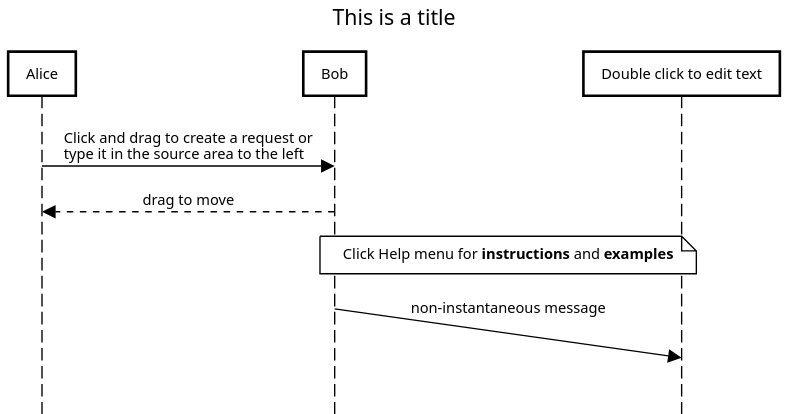
\includegraphics[width=0.8\textwidth]{../../assets/sequence-diagrams/StudentsSignsUp.png}
\end{figure}

\subsubsection{CompanySignsUp}

\subsubsection{UserLogsIn}

\begin{table}[H]
    \centering
    \begin{tabular}{|l|m{10cm}|}
        \hline \multicolumn{2}{|c|}{\textbf{UserLogsIn}} \\
        \hline \textbf{Actor} & Student, Company, University, Students\&Companies \\
        \hline \textbf{Entry condition} & User is registered \\
        \hline \textbf{Event flow} &
        \begin{enumerate}
            \item The user opens the log in page
            \item The platform shows the log in page
            \item The user enters its credentials and clicks the log in button
            \item The platform checks that the account exists and the credentials are correct
            \item The platform shows the home page
        \end{enumerate}
        \\
        \hline \textbf{Exit condition} & The user is logged in \\
        \hline \textbf{Exceptions} & The student is not registered \\
        \hline
    \end{tabular}
\end{table}

\begin{figure}[H]
    \centering
    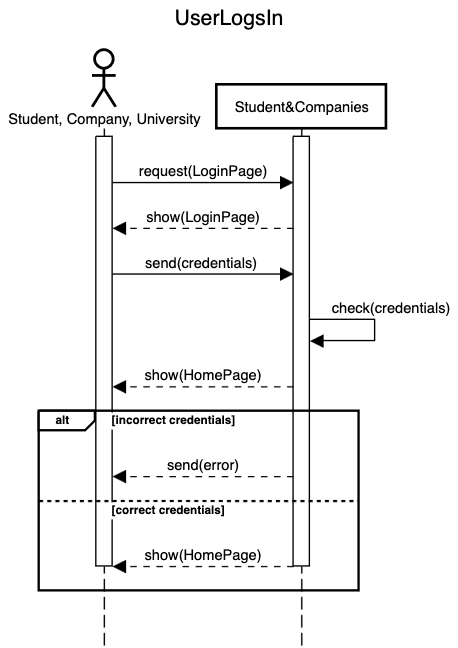
\includegraphics[width=0.5\textwidth]{../../assets/sequence-diagrams/UserLogsIn.png}
\end{figure}




\subsubsection{StudentUploadsCV}

\subsubsection{CompanyCreatesAdvertisement}

\subsubsection{StudentVisualizesAdvertisements}

\begin{table}[H]
    \centering
    \begin{tabular}{|l|m{10cm}|}
        \hline \multicolumn{2}{|c|}{\textbf{StudentVisualizesAdvertisements}} \\
        \hline \textbf{Actor} & Student, Students\&Companies \\
        \hline \textbf{Entry condition} & User is logged in \\
        \hline \textbf{Event flow} &
        \begin{enumerate}
            \item The user opens the home page
            \item The platform finds the advertisements that match the student profile
            \item The platform shows the home page with the advertisements
        \end{enumerate}
        \\
        \hline \textbf{Exit condition} & The user click on a advertisement or changhe the page \\
        \hline \textbf{Exceptions} & None \\
        \hline
    \end{tabular}
\end{table}

\begin{figure}[H]
    \centering
    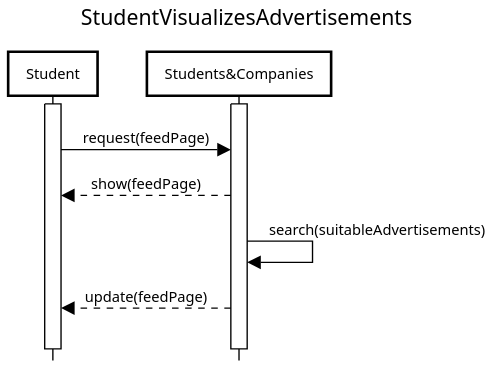
\includegraphics[width=0.5\textwidth]{../../assets/sequence-diagrams/StudentVisualizesAdvertisements.png}
\end{figure}




\subsubsection{CompanyVisualizesCandidates}

\subsubsection{CompanyCreatesQuestionnaire}

\subsubsection{StudentFillsQuestionnaire}
\begin{table}[H]
    \centering
    \begin{tabular}{|l|m{10cm}|}
        \hline \multicolumn{2}{|c|}{\textbf{StudentFillsQuestionnaire}} \\
        \hline \textbf{Actor} & Student, Company, Students\&Companies \\
        \hline \textbf{Entry condition} & User is logged in \\
        \hline \textbf{Event flow} &
        \begin{enumerate}
            \item The company creates a questionnaire
            \item The student opens the profile page
            \item The student fills the form in the profile page and clicks the submit button
        \end{enumerate}
        \\
        \hline \textbf{Exit condition} & The questionnaire button is no longer available \\
        \hline \textbf{Exceptions} & None \\
        \hline
    \end{tabular}
\end{table}

\begin{figure}[H]
    \centering
    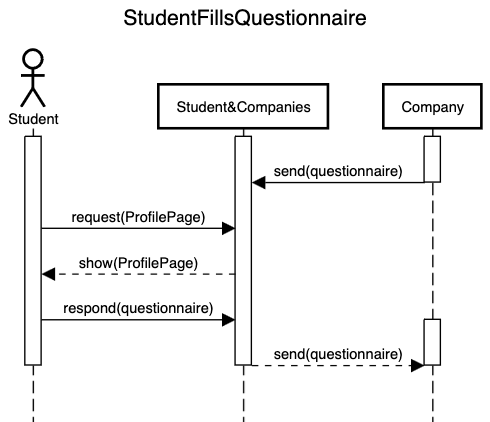
\includegraphics[width=0.5\textwidth]{../../assets/sequence-diagrams/StudentFillsQuestionnaire.png}
\end{figure}

\subsubsection{CompanyAcceptsStudentEnrollment}

\subsubsection{StudentVisualizesInternshipInformation}

\subsubsection{CompanyVisualizesInternshipsInformation}

\begin{table}[H]
    \centering
    \begin{tabular}{|l|m{10cm}|}
        \hline \multicolumn{2}{|c|}{\textbf{CompanyVisualizesInternshipsInformation}} \\
        \hline \textbf{Actor} & Company, Students\&Companies \\
        \hline \textbf{Entry condition} & Company is logged in \\
        \hline \textbf{Event flow} &
        \begin{enumerate}
            \item The company opens the profile page
            \item The company selects an internship from the list of all interships
            \item The system shows the internship information and the student enrolled
        \end{enumerate}
        \\
        \hline \textbf{Exit condition} & The company displays all the information \\
        \hline \textbf{Exceptions} & None \\
        \hline
    \end{tabular}
\end{table}

\begin{figure}[H]
    \centering
    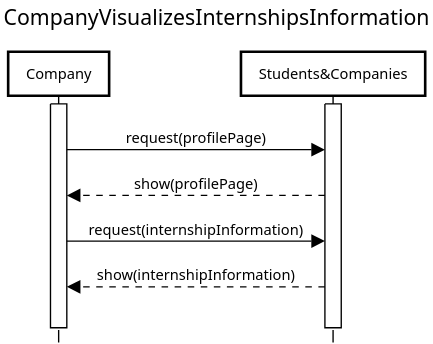
\includegraphics[width=0.5\textwidth]{../../assets/sequence-diagrams/CompanyVisualizesInternshipsInformation.png}
\end{figure}


\subsubsection{StudentSendsComplaint}

\subsubsection{CompanySendsComplaint}

\subsubsection{UniversityVisualizesComplaints}

\subsubsection{UniversityEndsInternship}

\subsubsection{InternshipExpires}

\subsubsection{StudentFillsFeedbackForm}

\subsection{Mapping}

\section{Performance requirements}

\subsection{Specific requirements}

\section{Design constraints}
\subsection{Standards compliance}
\subsection{Hardware limitations}
\subsection{Any other constraint}

\section{Software system attributes}
\subsection{Reliability}
\subsection{Availability}
\subsection{Security}
\subsection{Maintainability}
\subsection{Portability}